% !TEX encoding = UTF-8
% !TEX program = pdflatex
% !TEX spellcheck = it_IT

\documentclass[a4paper, 11pt]{article}

% sintassi
\usepackage[T1]{fontenc}
\usepackage[utf8]{inputenc}
\usepackage[english]{babel}
\DeclareUnicodeCharacter{00A0}{~}
\usepackage{fullpage}
%\usepackage[cochineal]{newtxmath}
%\usepackage{crimson,verbatim}
\usepackage[charter]{mathdesign}
\usepackage{textcomp}
\usepackage{color,soul,hyperref,mwe}

% matematica e chimica

\usepackage{siunitx,amsmath,bm,chemfig}
\newcommand{\ud}{\mathop{}\!\mathrm{d}}
\sisetup{detect-all,math-rm = \ensuremath}

\setatomsep{2em}

\newcommand\setpolymerdelim[2]{\def\delimleft{#1}\def\delimright{#2}} 
\def\makebraces[#1,#2]#3#4#5{% 
\edef\delimhalfdim{\the\dimexpr(#1+#2)/2}% 
\edef\delimvshift{\the\dimexpr(#1-#2)/2}% 
\chemmove{% 
\node[at=(#4),yshift=(\delimvshift)] {$\left\delimleft\vrule height\delimhalfdim depth\delimhalfdim 
width0pt\right.$};% 
\node[at=(#5),yshift=(\delimvshift)] 
{$\left.\vrule height\delimhalfdim depth\delimhalfdim 
width0pt\right\delimright_{\rlap{$\scriptstyle#3$}}$};}} 
\setpolymerdelim()

% tabelle e grafica
\usepackage{booktabs,graphicx,subfig,caption,pdfpages}
\captionsetup{font=small,
	format=hang,
	justification=centering,
	singlelinecheck=true,
	labelfont={sf,bf}	
}
\usepackage{float}
\floatstyle{plaintop}
\restylefloat{table}
\usepackage{multirow}
\usepackage{fancyhdr}
\pagestyle{fancy}
\fancyhead[LE,RO]{\textsl{\rightmark}}
\fancyhead[LO,RE]{\nouppercase{\leftmark}}
\fancyfoot[C]{\thepage}
\usepackage[margin=1in,headsep=.3in]{geometry}
\usepackage[suftesi]{frontespizio}
\usepackage{xparse}
\setlength\parindent{0pt}

\newenvironment{chapterabstract}{%
  \par\nobreak\noindent
  \textbf{\textit{Abstract}\hrulefill}\nobreak
  %\small
  \noindent\ignorespaces
}{%
  \par\nobreak\normalsize
  \vskip-\ht\strutbox\noindent
  \textbf{\hrulefill}%
}
\makeatletter
\NewDocumentCommand\headerspdf{ O {pages=-} m }{% [options for include pdf]{filename.pdf}
  \includepdf[%
    #1,
    pagecommand={\thispagestyle{fancy}},
    scale=1,
    ]{#2}}
\NewDocumentCommand\secpdf{somO{1}m}{% [short title]{section title}[page specification]{filename.pdf} --- possibly starred
  \clearpage
  \thispagestyle{fancy}%
  \includepdf[%
    pages=#4,
    pagecommand={%
      \IfBooleanTF{#1}{%
        \section*{#3}}{%
        \IfNoValueTF{#2}{%
          \section{#3}}{%
          \section[#2]{#3}}}},
    scale=.65,
    ]%
    {#5}}
\makeatother

\begin{document}

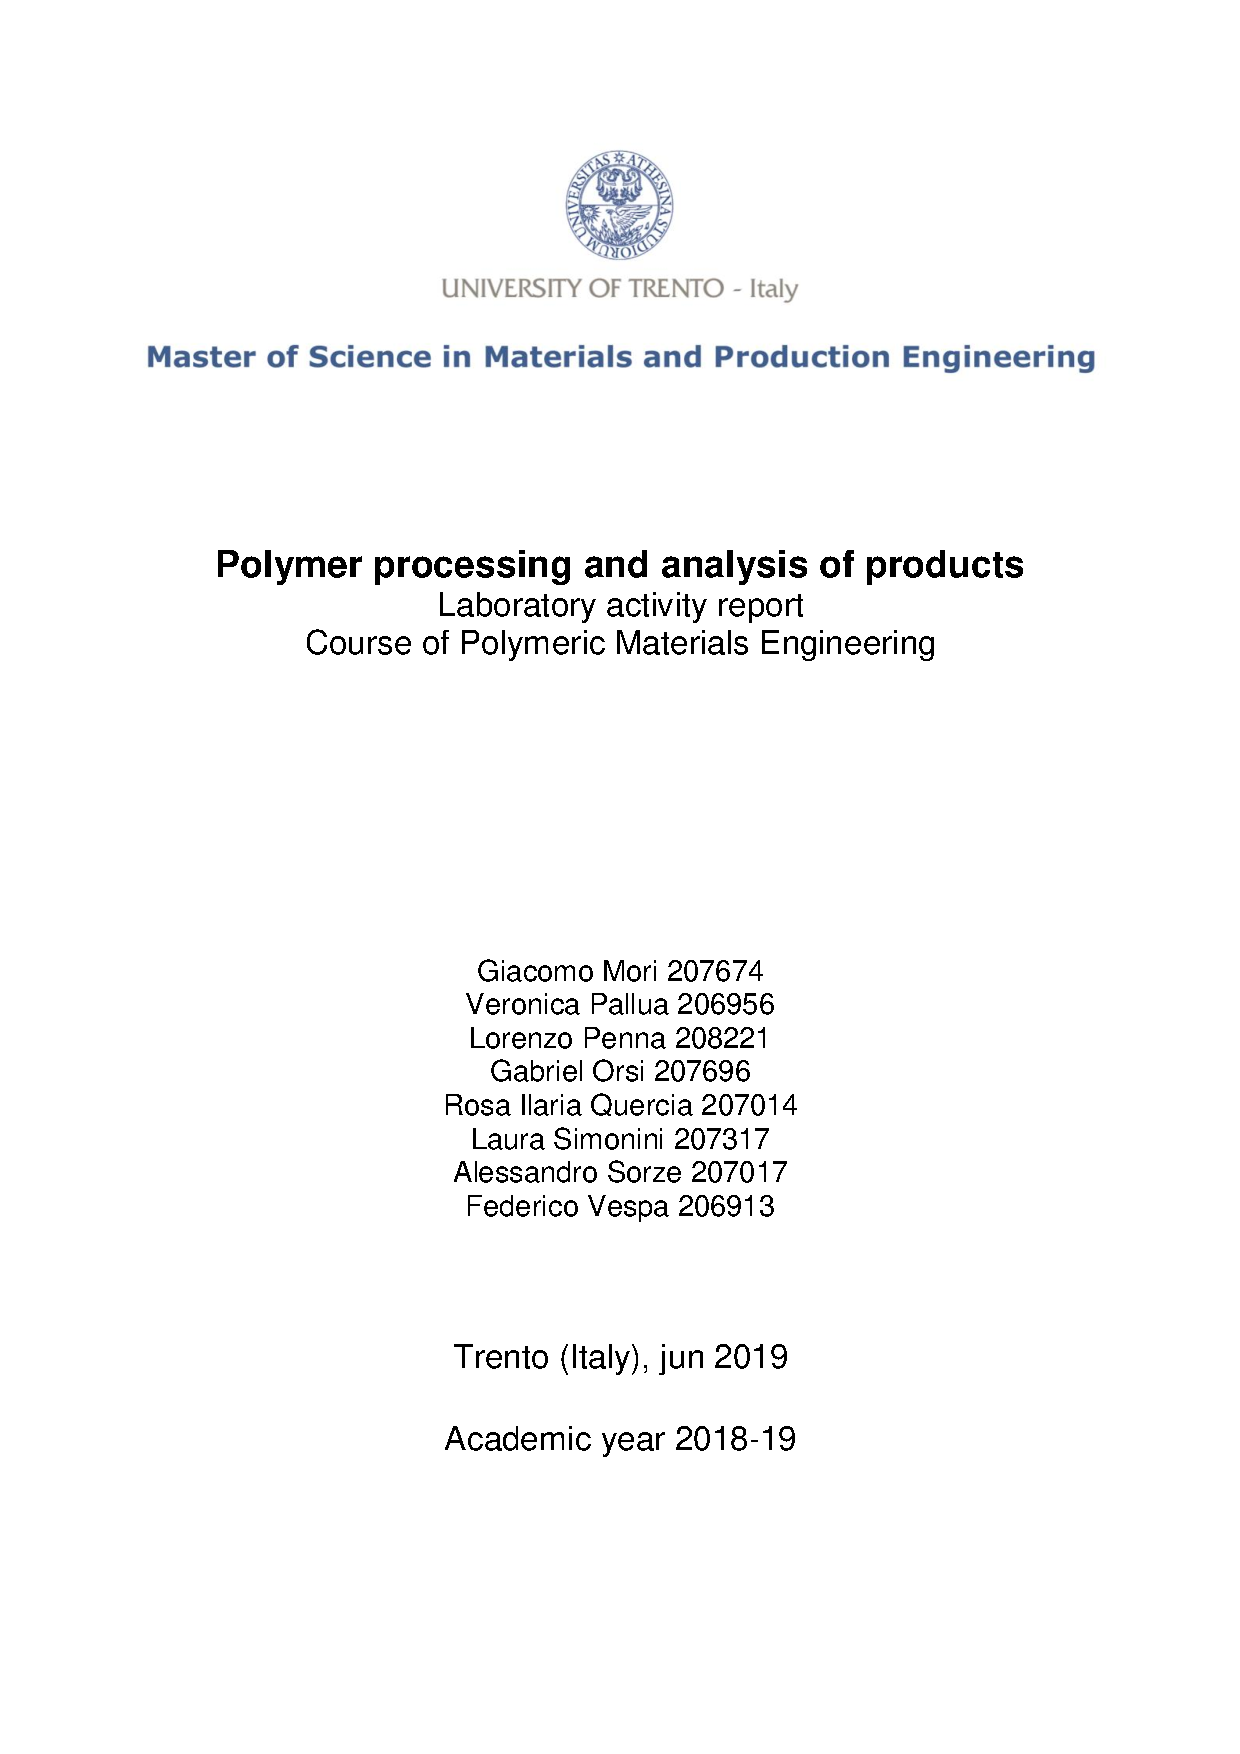
\includepdf{frontespizio4.pdf}

\begin{chapterabstract}

Lorem ipsum dolor sit amet, consectetur adipiscing elit. Nulla hendrerit, lorem feugiat dignissim congue, justo metus eleifend urna, a iaculis turpis purus vel ante. Maecenas vitae augue iaculis elit blandit lobortis et et neque. Fusce lacinia augue fringilla nisi consequat dapibus. Quisque molestie volutpat commodo. Suspendisse porta velit facilisis interdum tempus. Donec accumsan, justo a eleifend ullamcorper, leo nisi blandit nibh, eu scelerisque metus odio in tellus. Maecenas eget varius metus, at fermentum lectus. Maecenas eget condimentum mi. Nulla facilisi. Sed at sagittis lectus, sed pulvinar ligula.

\end{chapterabstract} 

\section{Introduction}

\section{Materials and methods}

Two types of Polypropylene (PP) have been poured together in order to obtain a mixture with higher properties with respect to the matrix. For our purpose 15\% in weight of flame retardant PP pellet has been added to isotactic PP (PPH-B-10-FB). In Figure \ref{fig:datasheet} is reported the technical datasheet of PPH-B-10-FB.
For compression molding a stainless steel plates with a frame of $12\times 12\, \text{mm}^2$ has been filled with 34 g of the mixture composed by 27.22 g of isotactic PP and 6.68 g of flame retardant PP. 
For injection compounding 40 g of the mixture have been weighed. In this case the misture was composed by 34.01 g of isotactic PP and 5.99 g of flame retardant PP.
\begin{figure}[h!]
	\centering
	{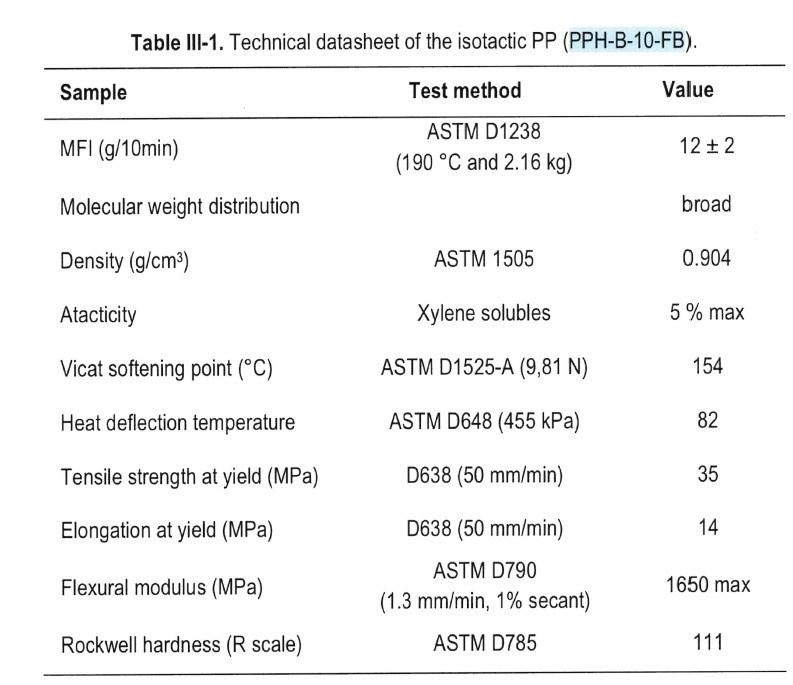
\includegraphics[scale=0.6]{datasheetPP}}
	\captionsetup{justification=centering}
	\caption{Technical datasheet of PPH-B-10-FB}
	\label{fig:datasheet}
\end{figure}\\

\section{Experimental activity}

\subsection{Compression molding}

Prepared amount of polypropylene mixture has been used for compression molding process. A press by Carver has been used, as illustrated in Figure \ref{fig:press}. 
\begin{figure}[htp]
	\centering
	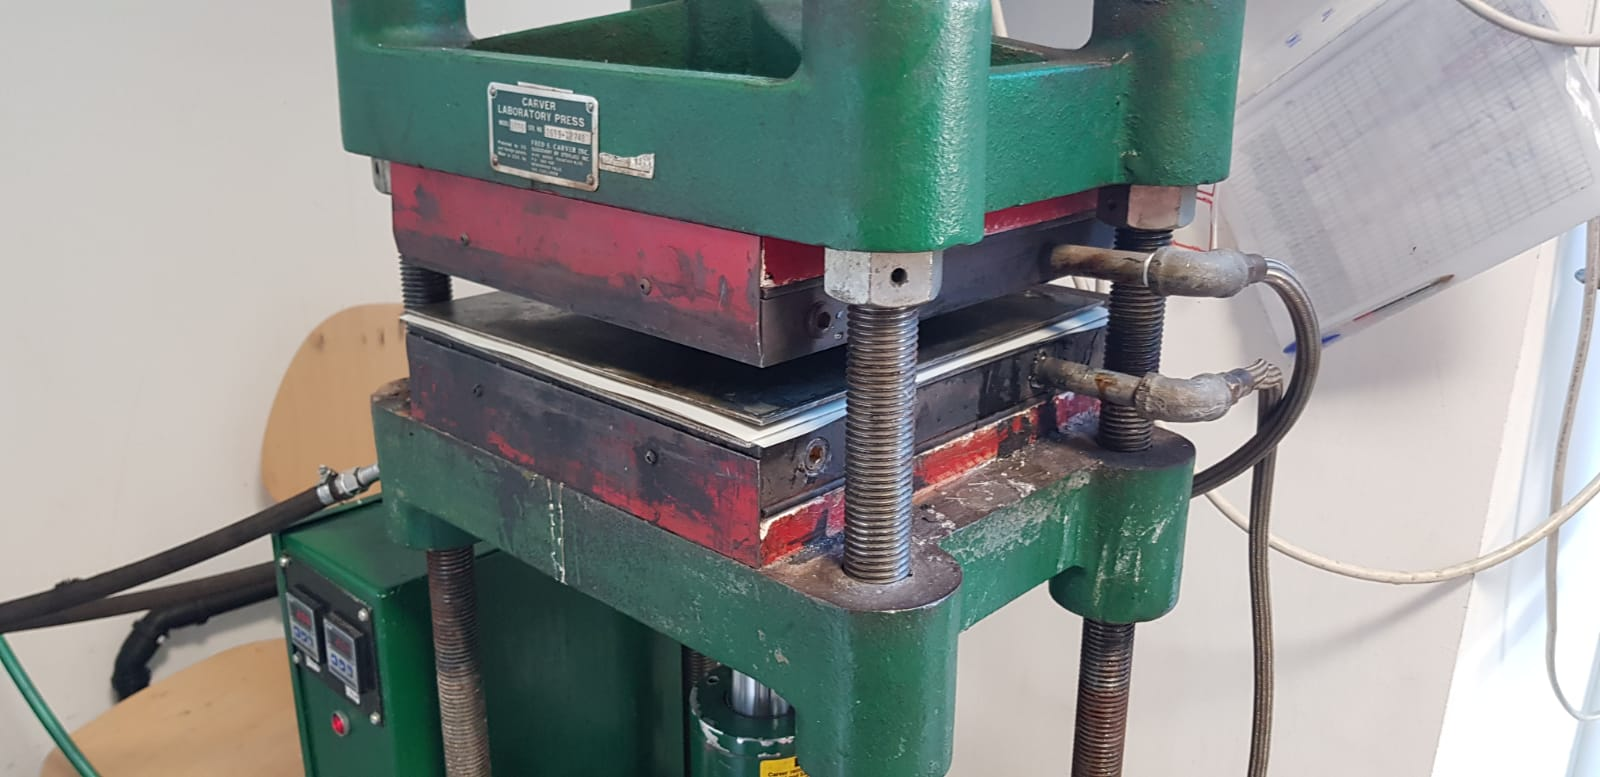
\includegraphics[scale=0.2]
	{PHOTO-2019-05-23-17-38-03.jpg}
	\label{fig:press}
	\caption{Carver press for compression molding.}
\end{figure}\\
The material to be pressed is put between two stainless steel plates, one having a frame of $12\times 12\, \text{mm}^2$ in order to produce a square plate of some mm of thickness. To avoid any adhesion with the plates, that are used to evenly distribute the pressure and to confine the melt (since the press is able to provide heat), two Mylar${^\text{\textregistered}}$ foils have been put in between the steel and the material. The press has been set to produce a pressure of 8 tons, equivalent to 5.45 MPa, in the frame. The material has undergone an heat treatment under this pressure of 200°C for 10 minutes. After this, the press has been cooled with water circulating in a refrigerating circuit inside of it and the molded piece extracted. Produced plate is then visually analyzed and weighted in order to estimate weight losses. \par 


\subsubsection{Compounding (internal mixer)}

The process has been carried out with the instrument Thermo Haake Rheomix 600, where the polypropylene mixture undergoes a thermal treatment of $200^\circ$C for 10 minutes. Rotation speed has been set at 40 rpm.
\begin{figure}[htp]
	\centering
	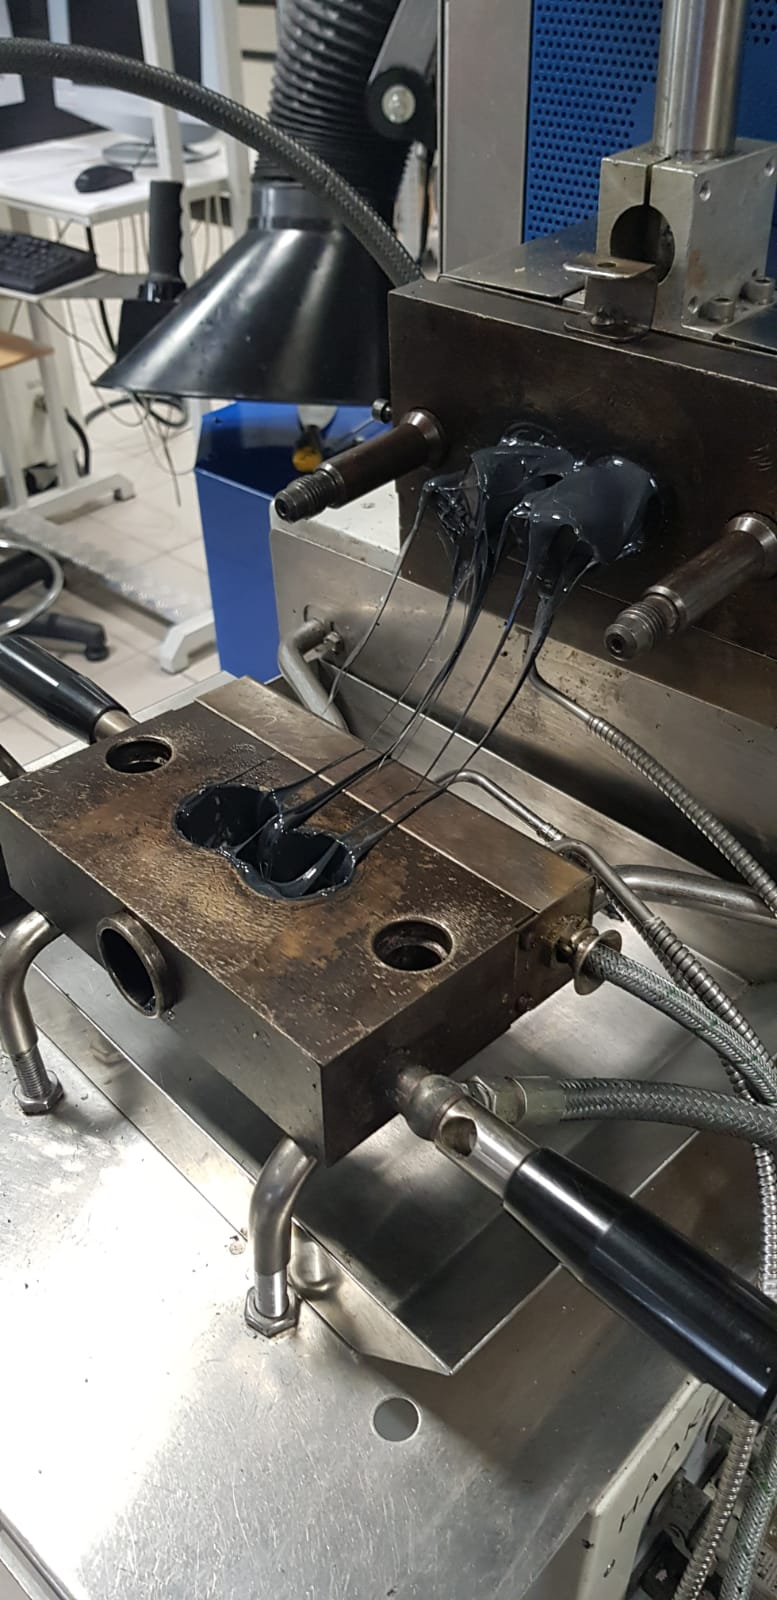
\includegraphics[scale=0.3]
	{PHOTO-2019-05-23-17-37-35.jpg}
	\label{fig:rheo}
	\caption{Rheomix 600 after usage. Remains of polypropylene mixture are visible.}
\end{figure}\\
The product obtained by this process has then been subjected to compression molding, using the same parameters as Plate 1. Tangential speed of the compounder is estimated to 0.082 m/s.

\subsubsection{Production of dumbbell specimens}

After the analysis of the plate, this has been cut to obtain ISO 527-1BA shaped specimens, that are used in another laboratory activity.     

\subsection{Injection molding: sample evaluation}
Different specimens of unknown polymeric materials have been analysed and identified. They have been produced by injection molding according to specific standards (ISO and ASTM):
\begin{itemize}
\item ISO 10.0 $\times$ 4.0 $\times$ 172 (mm);
\item ASTM 12.7 $\times$ 3.3 $\times$ 165 (mm);
\end{itemize}

In Table \ref{tab:materials} the types of samples are divided by standard (ASTM and ISO). 
\begin{table}[htp]
	\centering
	$
	\begin{array}{ll}
	\toprule
	\textbf{ASTM dumbbell} & \textbf{ISO dumbbell}  \\
	\midrule
	\text{ABS} & \text{POM bi-injected}\\
        \text{COC} & \text{PA11 mono-injected}\\
	\text{PP} & \text{PP-GF 30 (white) and PP-GF35 (black)}\\
	\text{HDPE Eltex yellow} & \text{PA6-GF50}\\
	\text{PE/PP blend} & \text{}\\
	\text{PA11} & \text{}\\
	\bottomrule
	\end{array}
	$
	\caption{Materials used in sample evaluation}
	\label{tab:materials}
\end{table}

Size of all specimens and the mold cavity have been measured through a caliper in order to evaluate the shrinkage after the process according to Equation \ref{eq:shr}.
\begin{equation}
\text{shrinkage} = \frac{\Delta x}{x_0}
\label{eq:shr}
\end{equation}

Where $\Delta x$ is the difference between the initial and final dimension (lenght, width and thickness) and $x_0$ is the initial dimension (lenght, width and thickness). 

ASTM samples (with sprue and bar) have been weighted through the balance Mettler PM 4600 in order to compare the total weight and polymer density (taken from literature~\cite{handbook}).

\subsection{Filament analysis}

Different fibers provided by University of Trento (polypropylene, see Materials and Methods) have been analyzed: in particular the diameter of six different filament samples have been measured in order to predict their mechanical properties in function of the draw ratio and the process parameters. 
Diameters have been taken using micrometer \textbf{[modello]}. The filament linear density (titer, fineness) is calculated accordingly to the Equation \ref{eq:titer}. 
\begin{equation}
	t = \rho \cdot A
	\label{eq:titer}
\end{equation}
where $t$ is the titer expressed in dtex, $\rho$ is the density and $A$ is the cross-section of the fiber, considered as circular. Titer in denier is found multiplying $t$ by a factor 0.9. The apparent draw ratio $DR$ is calculated using Equation \ref{eq:DR}. 
\begin{equation}
	DR = \Bigl(\frac{D_{max}}{D_{min}}\Bigr)^2
	\label{eq:DR}
\end{equation}
where $D_{max}$ is the maximum diameter of the collected fibers while $D_{min}$ is the minimum diameter. The fiber strength $T_{as}$ (tenacity as spun) is measured in $\frac{\text{cN}}{\text{dtex}}$ and it's calculated accordingly to the Equation \ref{eq:tenacity}. 
\begin{equation}
	T_{as} = \frac{\sigma_Y}{100\cdot \rho}
	\label{eq:tenacity}
\end{equation}
The tenacity after drawing $T_{DR}$ is given by Equation \ref{eq:tenacity2}. 
\begin{equation}
	T_{DR} = T_{as}\cdot DR
	\label{eq:tenacity2}
\end{equation}
The tensile strength $\sigma_b$ of the fibers is calculated accordingly to Equation \ref{eq:sigma}.
\begin{equation}
	\sigma_{b} = T_{DR}\cdot \rho \cdot 100
	\label{eq:sigma}
\end{equation}
where $\rho$ is expressed in g/cm$^3$. 

\newpage

\section{Results and discussion}

\subsection{Compression molding}

The mold before and after pressing is reported in Figure \ref{fig:beforeafter}. 

\begin{figure}[htp]
	\centering
	\subfloat[][]
	{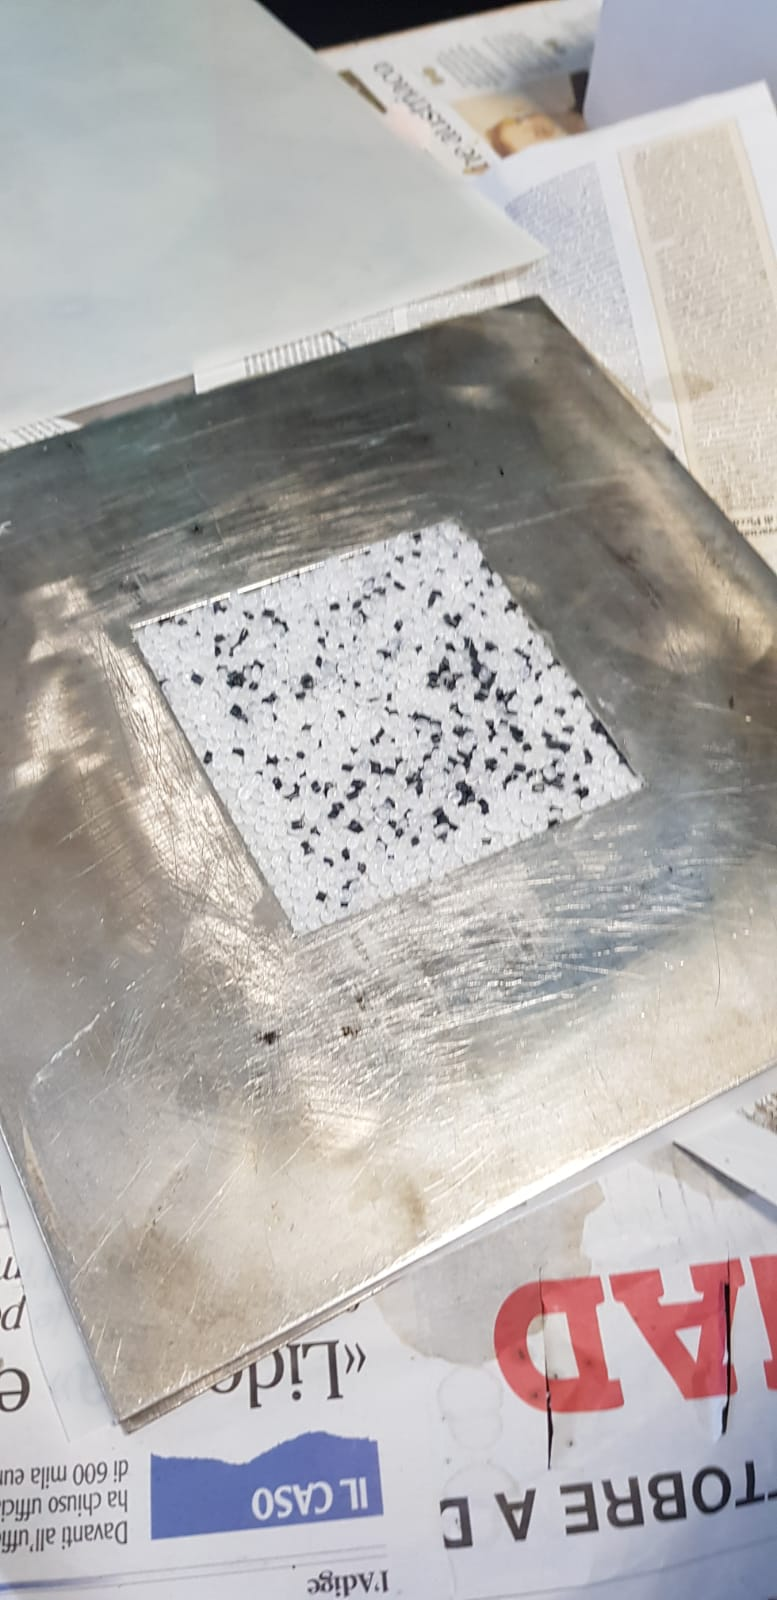
\includegraphics[scale=0.2]{PHOTO-2019-05-23-17-38-02.jpg}} \qquad 
	\subfloat[][]
	{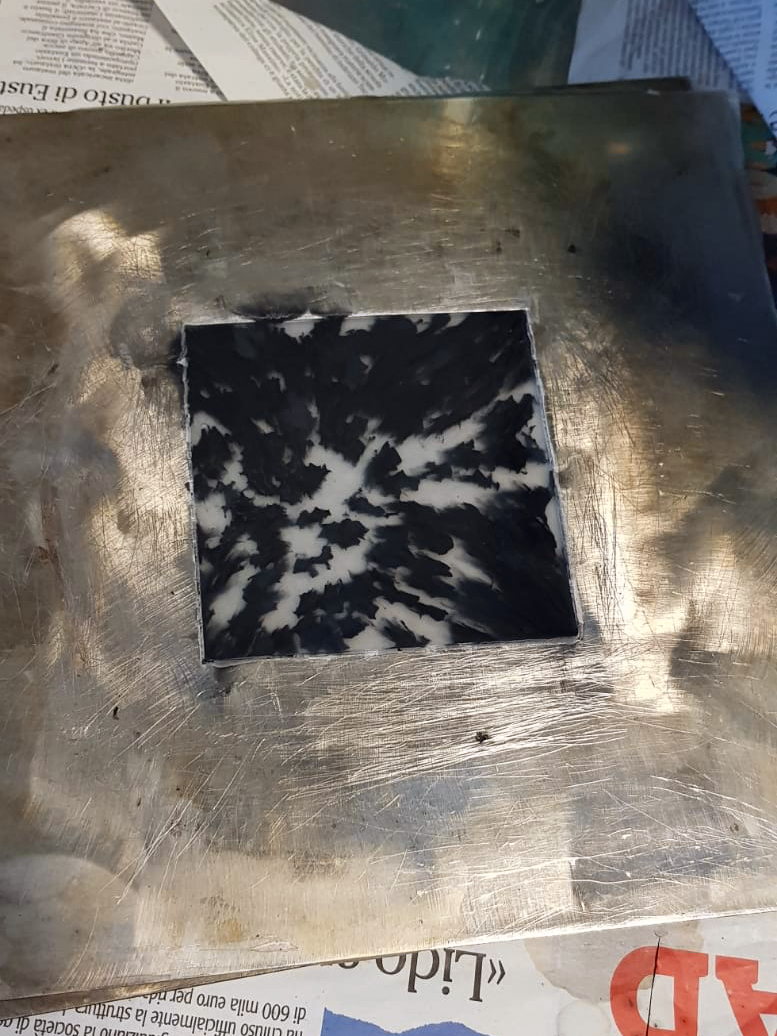
\includegraphics[scale=0.2]{PHOTO-2019-05-23-17-38-6.jpg}}
	\label{fig:beforeafter}
	\caption{Mold (a) before and (b) after compression.}
\end{figure}

The produced plate after manual mixing is illustrated in Figure \ref{fig:plate1}. 

\begin{figure}[htp]
	\centering
	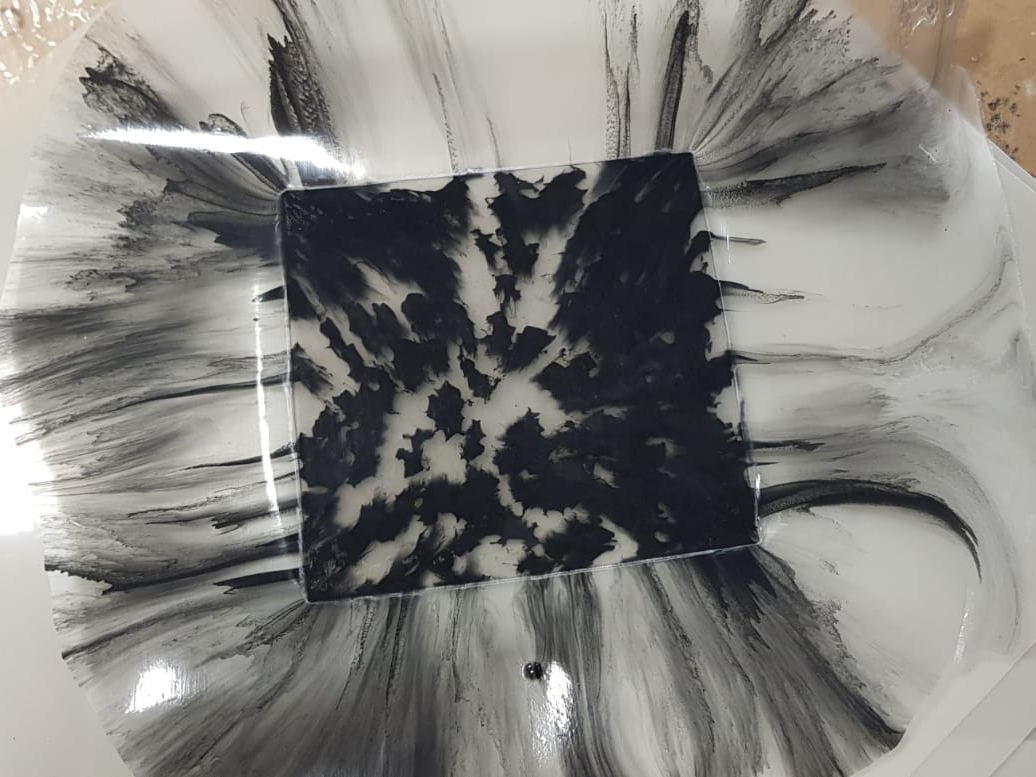
\includegraphics[scale=0.2]
	{PHOTO-2019-05-23-17-38-7.jpg}
	\label{fig:plate1}
	\caption{Plate produced in compression molding.}
\end{figure}

As it can be easily noted, the distribution of black PP in the white one is absolutely non-homogeneous, typical consequence of a manual mixing of the pellets (without any homogenization mixing in between). The other evident property of the pressed plate is the flash of melt outside of the mold: this is due to the too high amount of polymer inserted in the mold. 
The weights of the product before and after compression are reported in Table \ref{tab:weights_compression}. 

\begin{table}[htp]
	\centering
	$
	\begin{array}{ccc}
	\toprule
	\textbf{Mixture mass}\,\text{(g)} & \textbf{Plate mass}\,\text{(g)} & \textbf{Variation}\,\text{(\%)} \\
	\midrule
	34.00 & 32.50 & -4.41\\
	\bottomrule
	\end{array}
	$
	\caption{Mass of the sample before and after pressing.}
	\label{tab:weights_comparison}
\end{table}

\subsubsection{Compounding (Internal Mixer)}

A comparison between plates after compression molding si reported in Figure \ref{fig:plates}.
\begin{figure}[htp]
	\centering
	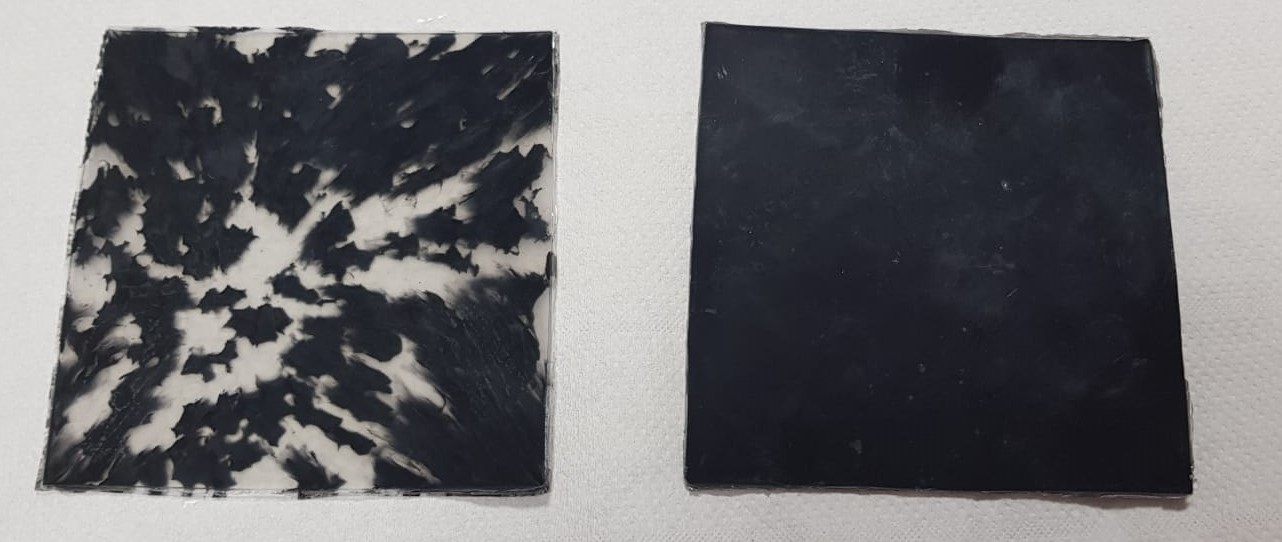
\includegraphics[scale=0.4]
	{PIATTI.jpg}
	\label{fig:plates}
	\caption{Compressed plates: plate 1 (from pellets) at left and plate 2 (from compounding) at right.}
\end{figure}\\
It can be seen that subjecting the sample to compounding before compression molding, a better homogeneity can  be reached.
The weights of the product before and after compression are reported in Table \ref{tab:weights_comparison}.

\begin{table}[htp]
	\centering
	$
	\begin{tabular}{cccc}
	\toprule
	\textbf{Sample} & \textbf{Mixture mass}\,\text{(g)} & \textbf{Plate mass}\,\text{(g)} & \textbf{Variation}\,\text{(\%)} \\
	\midrule
	1 & 34.00 & 32.50 & -4.41\\
	2 & 32.05 & 30.50 & -4.84\\
	\bottomrule
	\end{tabular}
	$
	\caption{Mass of the samples before and after pressing.}
	\label{tab:weights_comparison}
\end{table}

The table shows that the weight variation is slighty highier, that can be explained by the more difficult preparation of the sample before compression, due to its volume distribution.

\newpage

\subsubsection{Production of dumbbell specimens}

In Figure \ref{fig:spec}-a the dumbbell specimens produced in compression molding without compounding are displayed. As it can be seen, these specimens are characterized by low isotropy and homogeneity of the mixture. This will be a probable issue when mechanically testing and in resistance to flame propagation. Since the flame retardant is a weakener of strength (it introduces organics with poor adhesion and thus stress intensifiers), these specimens may have higher deformation at break than the more homogeneous ones produced in melt compounding, showed in Figure \ref{fig:spec}-b.
\begin{figure}[htp]
	\centering
	\subfloat[][]
	{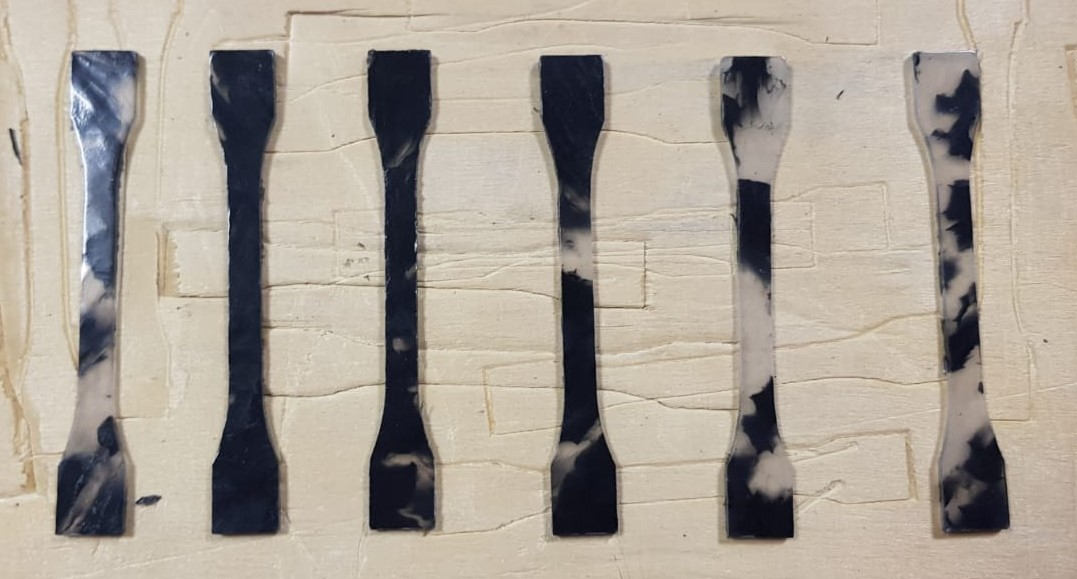
\includegraphics[scale=0.34]
	{PHOTO-2019-05-23-17-37-11.jpg}} \qquad
	\subfloat[][]
	{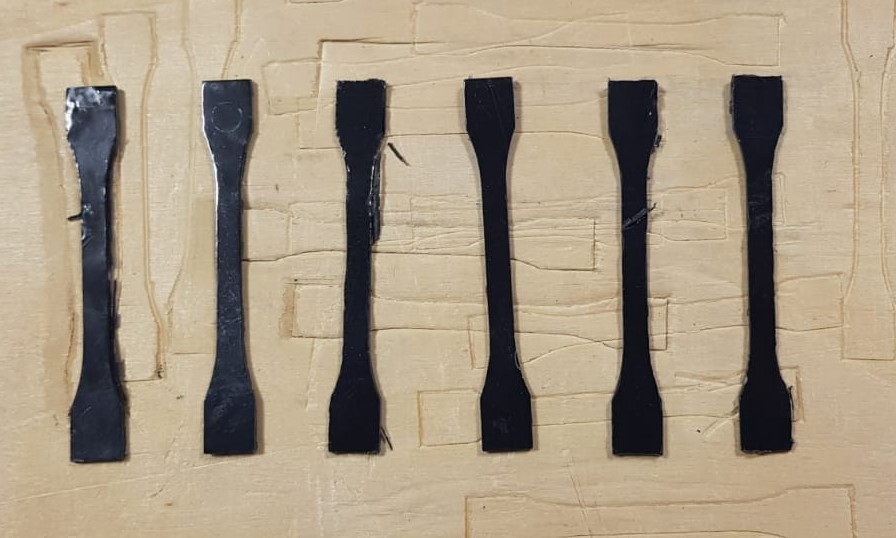
\includegraphics[scale=0.4]
	{PHOTO-2019-05-23-17-37-13.jpg}} 
	\label{fig:spec}
	\caption{Produced specimens from compression molding plate after compounding.}
\end{figure}

\newpage

\subsection{Injection molding: sample evaluation}

ISO specimens are reported in Figure \ref{fig:ISO}.

\begin{figure}[htp]
\centering
\subfloat[][]
{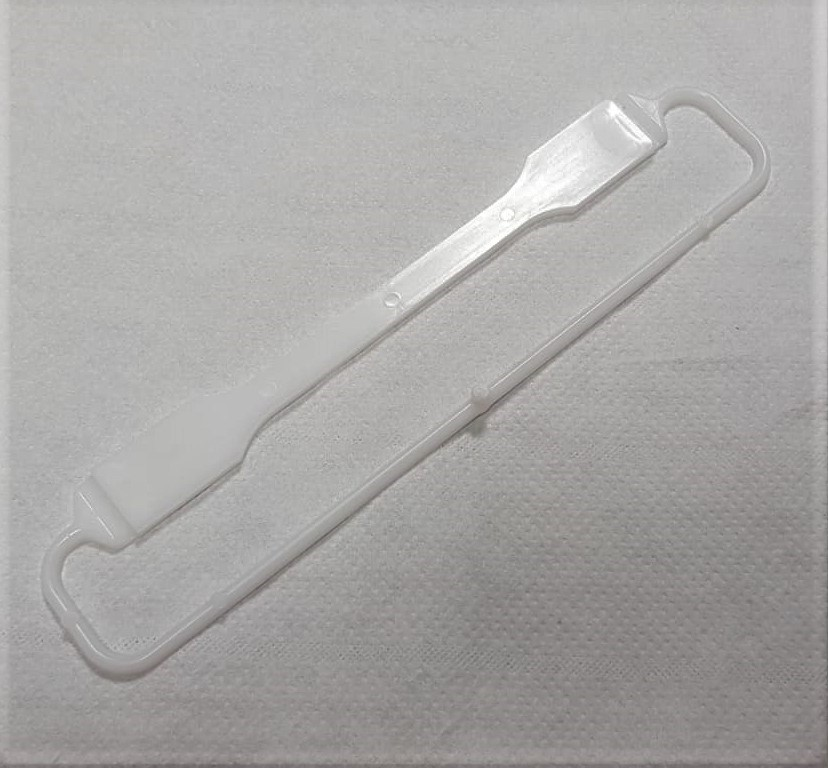
\includegraphics[scale=0.2]{POM}} \qquad
\subfloat[][]
{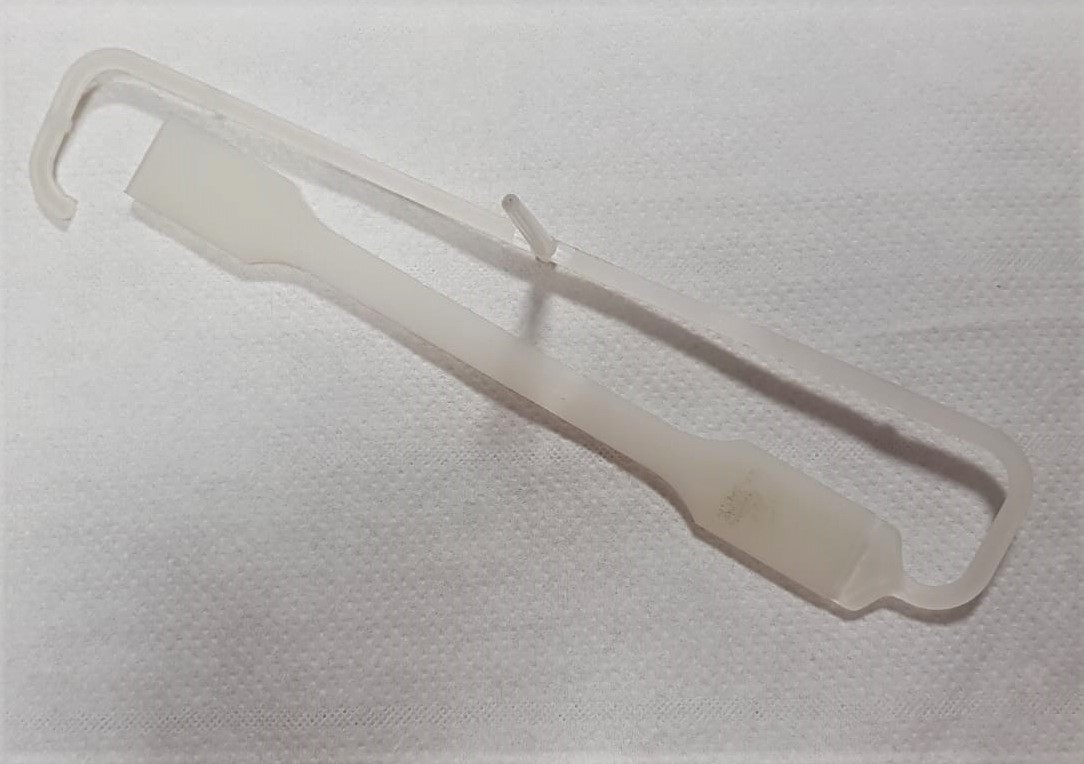
\includegraphics[scale=0.2]{PA11ISO}} \\
\subfloat[][]
{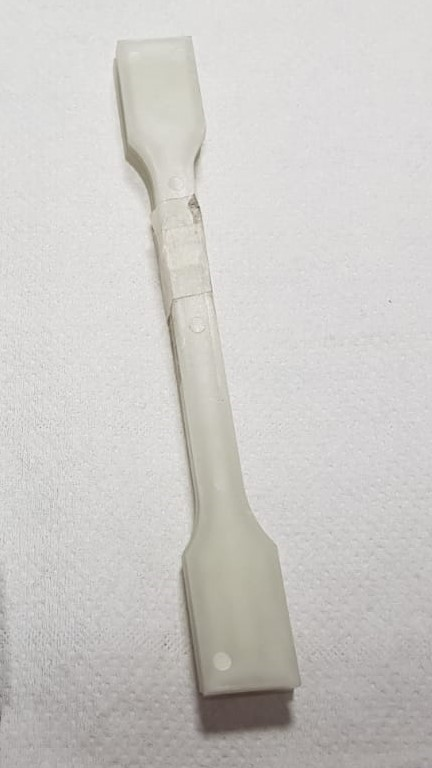
\includegraphics[scale=0.25]{PPW}} \qquad
\subfloat[][]
{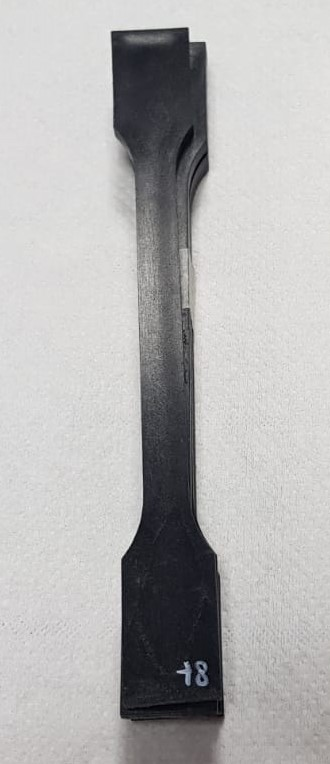
\includegraphics[scale=0.25]{PPB}} \qquad
\subfloat[][]
{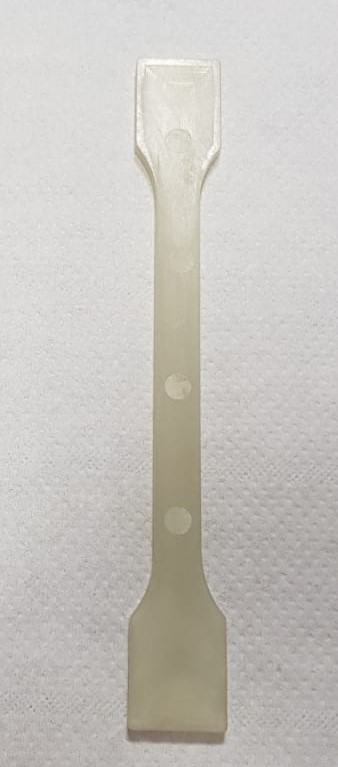
\includegraphics[scale=0.25]{PA6GF}}
\captionsetup{justification=centering}
\caption{ISO samples: a) POM; b) PA11; c) PP-GF30; d) PP-GF35; e) PA6-GF50. }
\label{fig:ISO}
\end{figure}

In Table \ref{tab:ISO} different types of ISO specimens are classified with their sizes.

\begin{table}[htp]
\centering
$
\begin{array}{llll}
\toprule
\textbf{Figure} & \textbf{Material} & \textbf{Size}\,(\text{mm}) & \textbf{Description} \\
\midrule
\text{a} & \text{POM} & 9.74\times 3.94\times 167.06 & \text{white and presence of cold junction}\\
\text{b} & \text{PA11} & 9.86\times 4.05\times 168.98 & \text{opaque and white}\\
\text{c} & \text{PP-GF30} & 9.88\times 4.00\times 172.11 & \text{white and stiff}\\
\text{d} & \text{PP-GF35} & 9.80\times 4.00\times 171.86 & \text{black and stiff}\\
\text{e} & \text{PA6-GF50} & 9.99\times 3.98\times 154.71 & \text{very stiff}\\
\bottomrule
\end{array}
$
\caption{ISO specimens and characteristics.}
\label{tab:ISO}
\end{table}

In Table \ref{tab:shISO} the values of the shrinkage of ISO samples are reported.

\begin{table}[h!]
\centering
$
\begin{array}{cccc}
\toprule
\textbf{Samples} & \textbf{Longitudinal shrinkage} & \textbf{Transversal shrinkage} & \textbf{Thickness} \\
\midrule
\text{POM} & 0.028 & 0.026 & 0.015 \\
\text{PA11} & 0.017 & 0.014 & -0.012 \\
\text{PP-GF30} & 0 & 0.012 & 0  \\
\text{PP-GF35} & 0.001 & 0.020 & 0  \\
\bottomrule
\end{array}
$
\caption{Shrinkage of ISO samples.}
\label{tab:shISO}
\end{table}

From Table \ref{tab:shISO} it can be noticed that in reinforced polymers the shrinkage is very small, almost negligible. The presence of glass fibers gives to polymers better dimensional stability during cooling. 

ASTM specimens are reported in Figure \ref{fig:ASTM}.

\begin{figure}[htp]
\centering
\subfloat[][]
{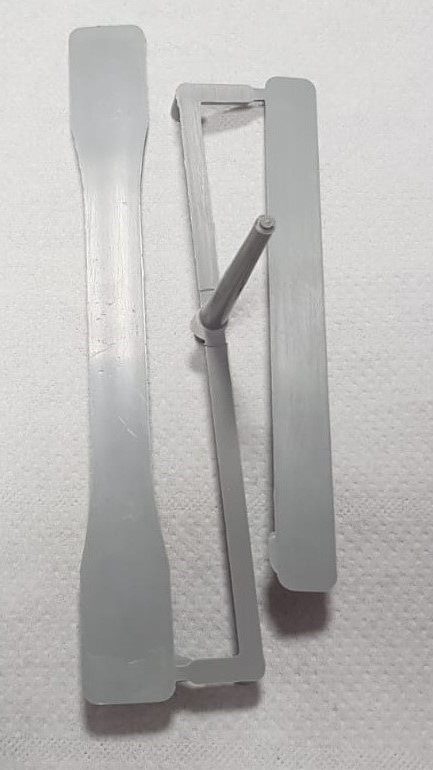
\includegraphics[scale=0.25]{ABS}} \qquad
\subfloat[][]
{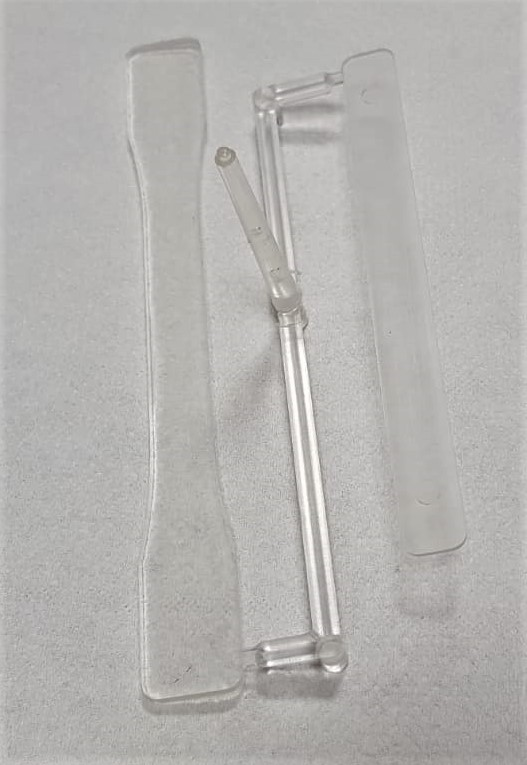
\includegraphics[scale=0.25]{COC}} \qquad
\subfloat[][]
{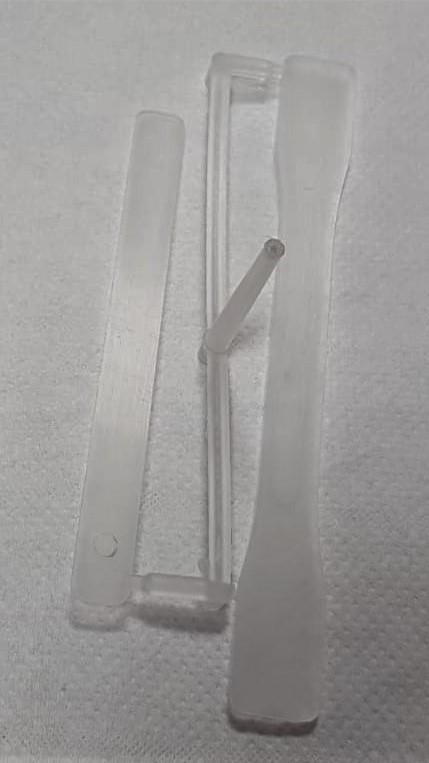
\includegraphics[scale=0.25]{PP}} \\
\subfloat[][]
{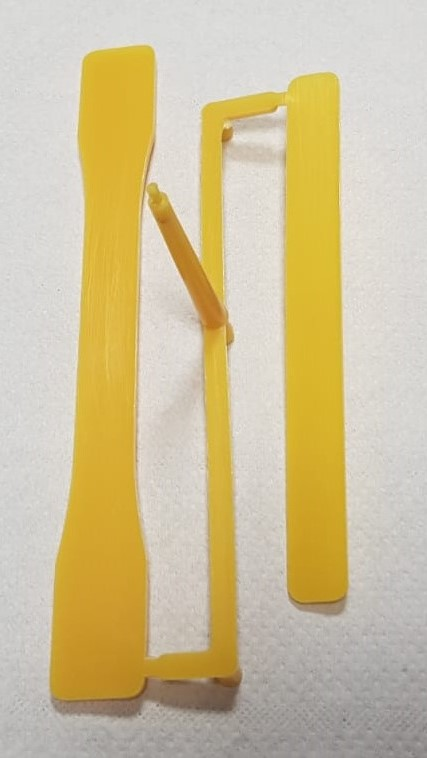
\includegraphics[scale=0.25]{HDPE}} \qquad
\subfloat[][]
{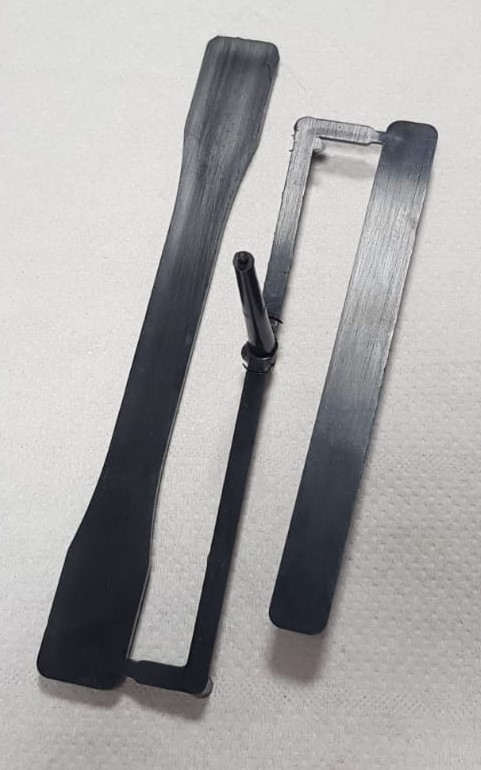
\includegraphics[scale=0.247]{PE-PP}} \qquad
\subfloat[][]
{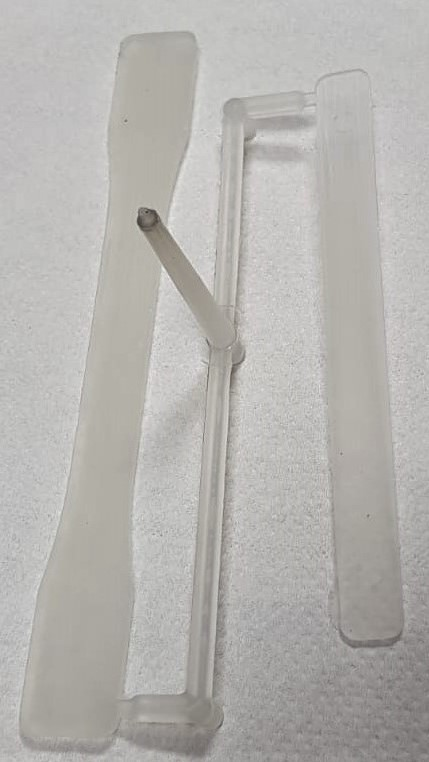
\includegraphics[scale=0.25]{PA11ASTM}} \\
\captionsetup{justification=centering}
\caption{ASTM samples: a) ABS; b) COC; c) PP; d) HDPE; e) PE/PP\ \text{blend}; f) PA11. }
\label{fig:ASTM}
\end{figure}

In Table \ref{tab:ASTM} different types of ASTM specimens are classified with their sizes.
\begin{table}[htp]
\centering
$
\begin{array}{lllll}
\toprule
\textbf{Figure} & \textbf{Material} & \textbf{Weight}\,(\text{g}) & \textbf{Size}\,(\text{mm}) & \textbf{Description} \\
\midrule
\text{a} & \text{ABS} & 14.78 & 12.77\times 3.27\times 163.55 & \text{grey and flexible}\\
\text{b} & \text{COC} & 14.07 & 12.64\times 3.30\times 164.04 & \text{transparent and glassy}\\
\text{c} & \text{PP} & 12.28 & 12.6\times 3.35\times 162.29 & \text{opaque and flexible} \\
\text{d} & \text{HDPE} & 12.73 & 12.54\times 3.33\times 160.0 & \text{yellow and very flexible} \\
\text{e} & \text{PE/PP}\ \text{blend} & 13.30 & 12.66\times 3.31\times 161.58 & \text{matt black and flexible} \\
\text{f} & \text{PA11} & 14.00 & 12.6\times 3.35\times 162.29 & \text{very similar to PP} \\
\bottomrule
\end{array}
$
\caption{ASTM specimens and characteristics.}
\label{tab:ASTM}
\end{table}
\\

\newpage

In Table \ref{tab:shASTM} the values of the shrinkage of ASTM samples are reported.

\begin{table}[htp]
\centering
$
\begin{array}{cccc}
\toprule
\textbf{Samples} & \textbf{Longitudinal shrinkage} & \textbf{Transversal shrinkage} & \textbf{Thickness} \\
\midrule
\text{ABS} & 0.009 & -0.006 & 0.009  \\
\text{COC} & 0.006 & 0.005 & 0 \\
\text{PP} & 0.016 & 0.003& -0.015 \\
\text{HDPE} & 0.030 & 0.013 & -0.009 \\
\text{PE/PP blend} & 0.021 & 0.002 & -0.003 \\
\text{PA11} & 0.016 & 0.003& -0.015 \\
\bottomrule
\end{array}
$
\caption{Shrinkage of ASTM samples.}
\label{tab:shASTM}
\end{table}

From Table \ref{tab:shASTM} it can be observed that semycristalline polymers (such as PP, HDPE, PA11) have higher values of shrinkage respect to amourphous polymers (such ABS and COC). Amorphous polymers have random arrangement of molecules that produces little volume changes thus lower shrinkage. \\
The higher values of longitudinal shrinkage in semycristalline polymers are partially compensated by the increase of the thickness (negative values of thickness shrinkage).

In Table \ref{tab:pesi} weights and densities of ASTM samples are reported.

\begin{table}[htp]
\centering
$
\begin{array}{ccc}
\toprule
\textbf{Samples} & \textbf{Weight}\,(\text{g}) & \textbf{Density}\,(\text{g/cm}^3) \\
\midrule
\text{ABS} & 14.78 & 1.04-1.12  \\
\text{COC} & 14.07 & 1.02 \\
\text{PP} & 12.28 & 0.85-0.94 \\
\text{HDPE} & 12.73 & 0.93-0.97 \\
\text{PE/PP blend} & 13.30 & 0.86-0.95 \\
\text{PA11} & 14.00 & 1.04 \\
\bottomrule
\end{array}
$
\caption{Weight and density of ASTM samples.}
\label{tab:pesi}
\end{table}

For PE/PP blend it has been considered a blend constituted by PE/PP $50\%$. From Table \ref{tab:pesi} it can be noticed that, for the same volume, weights of samples are in accordance with values of densities taken from literature~\cite{handbook}. 

\newpage

\subsection{Filament analysis}

Diameter and titer measurements are reported in Table \ref{tab:titer}.
\begin{table}[htp]
\centering
$
\begin{array}{cccc}
\toprule
\textbf{Sample} & \textbf{Diameter} \, (\text{µm}) & \textbf{Fineness}\, (\text{dtex}) & \textbf{Fineness} \, (\text{denier}) \\
\midrule
\text{F1} & 34 & 8.2 & 7.4 \\
\text{F2} & 87 & 53.7 & 48.3 \\ 
\text{F3} & 212 & 319.5 & 287.6 \\
\text{F4} & 248 & 437.0 & 393.3 \\
\text{F5} & 147 & 153.5 & 138.2 \\
\text{F6} & 41 & 11.9 & 10.7 \\
\bottomrule
\end{array}
$
\caption{Diameters and fineness measurements of collected fibers.}
\label{tab:titer}
\end{table}

Tenacities before and after drawing are reported in Table \ref{tab:tenacity}.
\begin{table}[htp]
\centering
$
\begin{array}{ccccc}
\toprule
\textbf{Sample} & \mathbf{T_{as}} \, (\frac{\text{cN}}{\text{dtex}}) & \textbf{DR} & \mathbf{T_{DR}}\, (\frac{\text{cN}}{\text{dtex}}) & \mathbf{\sigma_b} \, (\text{MPa})\\
\midrule
\text{F1} & 0.304 & 53.2 & 16.2 & 1464\\
\text{F2} & 0.304 & 8.1 & 2.5 & 223\\ 
\text{F3} & 0.304 & 1.4 & 0.4 & 38\\
\text{F4} & 0.304 & 1.0 & 0.3 & 28\\
\text{F5} & 0.304 & 2.8 & 0.9 & 78\\
\text{F6} & 0.304 & 36.6 & 11.1 & 1007\\
\bottomrule
\end{array}
$
\caption{Diameters and fineness measurements of collected fibers.}
\label{tab:titer}
\end{table}

Accordingly to literature~\cite{encyclopedia} high strength PP fibers can reach values of 2.6 GPa and 3.5\% deformation at break. Since tensile strength and deformation at break follow a hyperbolic envelope, by fitting these data with the generic equation of the hyperbole (only parameter is a constant), the following can be found, expressed in Figure \ref{fig:hyperbole}.
\begin{figure}[htp]
	\centering
	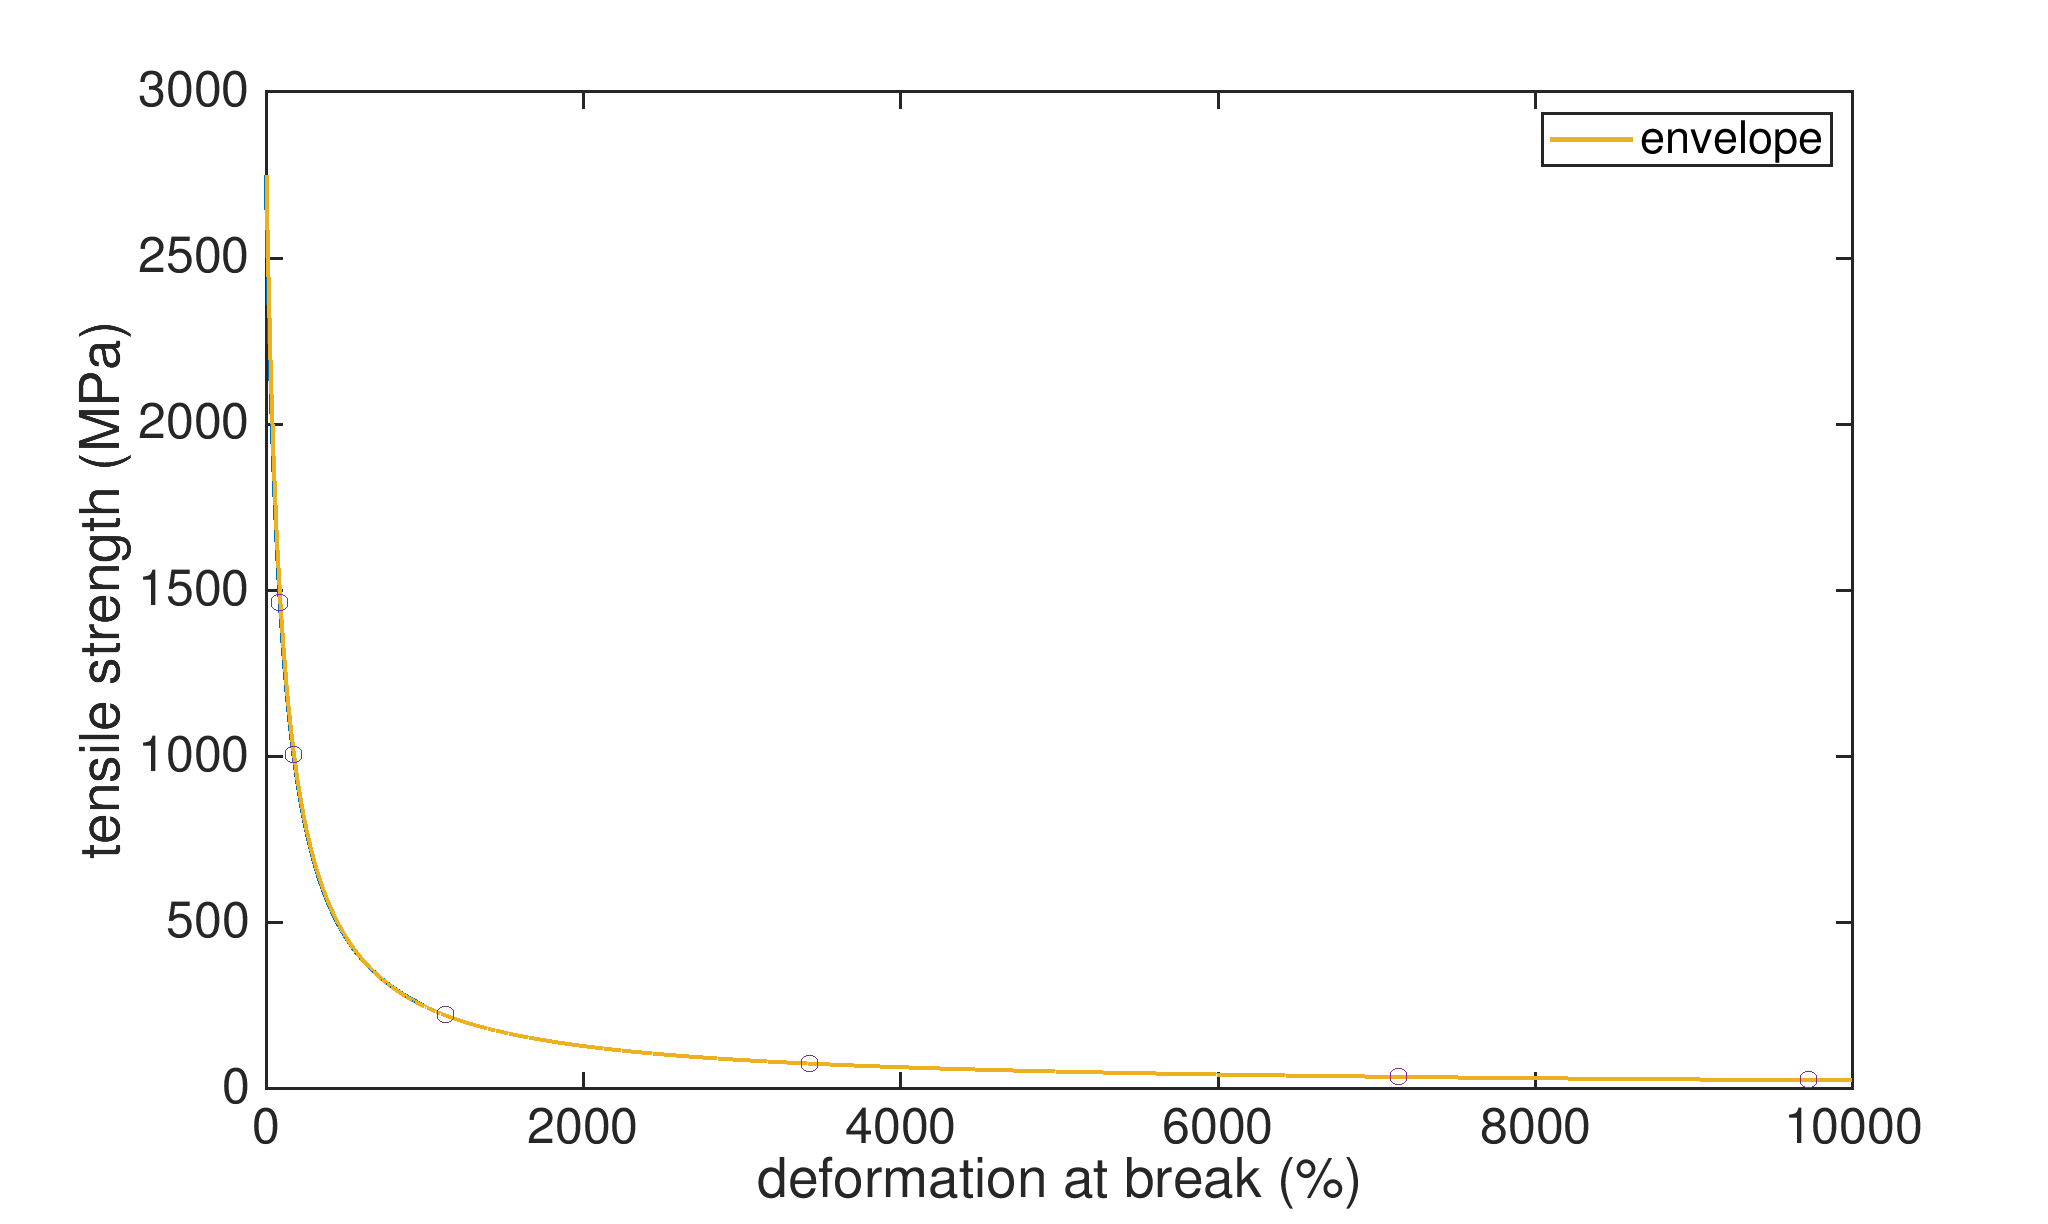
\includegraphics[scale=0.15]
	{hyperbole.png}
	\label{fig:hyperbole}
	\caption{Stress-strain relation for PP fibers.}
\end{figure}

As it can be easily noted, the distribution of black PP in the white one is absolutely non-homogeneous, typical consequence of a manual mixing of the pellets (without any homogenization mixing in between). The other evident property of the pressed plate is the flash of melt outside of the mold: this is due to the too high amount of polymer inserted in the mold. 



\begin{thebibliography}{1}

\bibitem{handbook} Polymer handbook, J. Brandrup, E.H. Immergut, fourth edition, Wiley 2003.
\end{thebibliography}
\end{document}